\section{$I \times J$ Table}
Suppose we have two categorical variables, $X$ and $Y$. The number of categories of $X$ is $I$ and the number of categories of $Y$ is $J$.

\begin{definition}[Contingency Table]
	A rectangular table having $I$ rows for the categories of $X$ and $J$
	columns for the categories of $Y$ has cells that display the $IJ$ possible
combinations of outcomes.
	
	Sometimes, it is also called frequency table or cross-classification table.
\end{definition}

Suppose the total number of observations $n = \sum_{i = 1}^{I} \sum_{j =1}^{J}n_{ij}$. 
\begin{figure}[H]
	\centering
	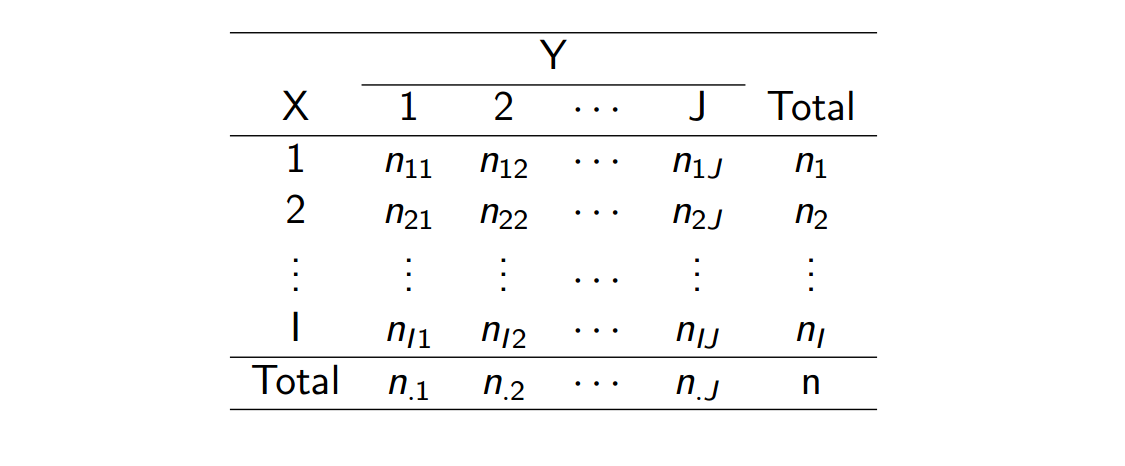
\includegraphics[width=0.7\linewidth]{fig/screenshot001}
	\caption{Example of $I \times J$ Contingency Table}
	\label{fig:screenshot001}
\end{figure}
